\chapter{Pyhop}

Para resolver un problema tenemos tres fases
\begin{enumerate}
   \item Modelato
   \item Planificación
   \item Ejecución
\end{enumerate}

El problema se define como una declaración de un nuevo estado del mundo (inicial), y una declaración de un objetivo.
El \textbf{dominio}, son las acciones disponibles, que se estructuran en dos niveles: tareas/operadores y métodos.


\begin{itemize}
	\item Información estática: no cambia durante la ejecución del
problema y que sirve de soporte. Por ejemplo: distancias
entre ciudades.
	\item Información dinámica: representa el estado actual del
mundo. Por ejemplo: cantidad de dinero disponible por el
agente en un momento determinado
\end{itemize}

\begin{figure}[htbp]
   \centering
   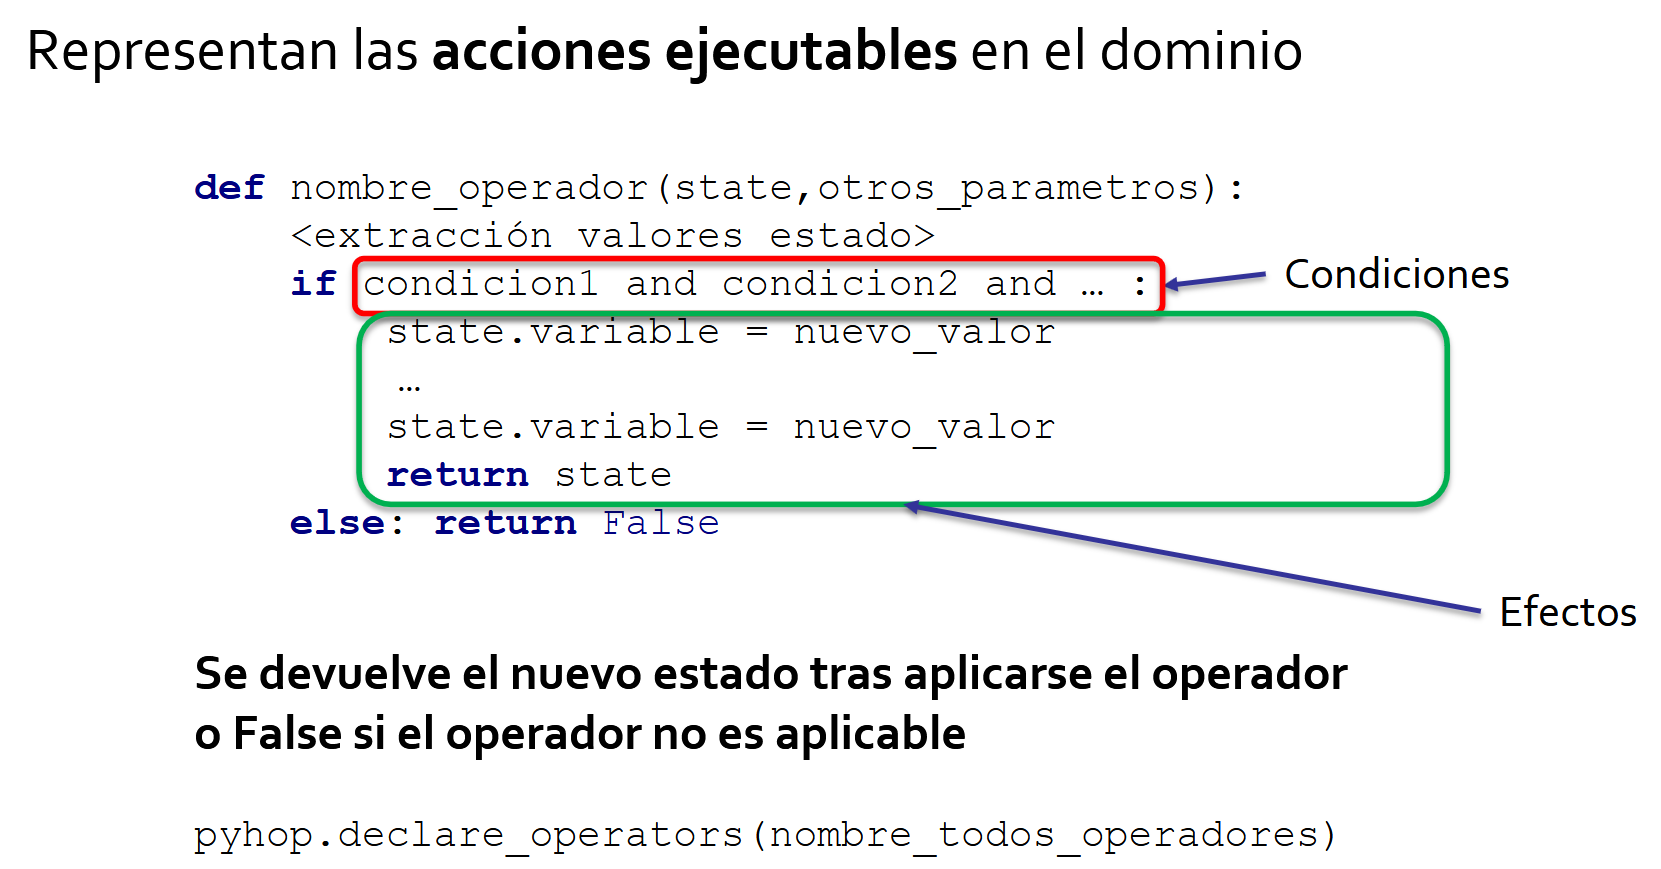
\includegraphics{images/03/operador.png}
   \caption{Como definir un operador en Pyhop}
   \label{fig:03/operador}
\end{figure}

% // TODO faltan ejemplos de Pyhop pero no pasa nada.

